\section{Homophily: \emph{"Birds of a feather flock together"}}
\label{sec:homophily}
%\vspace{-0.2cm}
%\begin{center} \emph{Birds of a feather flock together} \end{center}
%\vspace{0.1cm}

Homophily refers to the tendency of individuals to connect to similar others: two individuals (and thus their corresponding nodes in a social network) are more likely to be connected if they share common characteristics~\cite{mcpherson2001birds,lazarsfeld1954friendship}. The characteristics often considered are inherent to the individuals: they may represent their social status, their preferences, their interest, ... A related notion is the one of {\it assortativity}, which is slightly more general since it applies to any network, and not just social networks, and refers to the tendency of nodes in networks to be connected to others that are similar in some way.

A definition of homophily has been proposed in~\cite{la2010randomization}. However, this definition, which relies on a single characteristic (as age or gender), does not allow one to assess whether latent models for link prediction capture the homophily effect or not. We thus introduce a new definition of homophily below, which directly aims at this:
%
\begin{definition}[Homophily]
	Let $\mathcal{M}$ be a link prediction model as defined above and $s$ a similarity measure between nodes. We say that \emph{$\mathcal{M}$ captures the homophily effect} iff, $\forall (i,j,i',j') \in V^4$:
%
\begin{equation}
s(i,j) > s(i',j')  \implies \pr(y_{ij}=1 \mid \mathcal{M}) > \pr(y_{i'j'}=1  \mid \mathcal{M}) \nonumber
\end{equation}
%
A model which verifies this condition is said to be \emph{homophilic} under the similarity $s$.
\end{definition}
%
As one can note, this definition directly captures the effect "if two nodes are more similar, then they are more likely to be connected The similarity function assesses to which extent two nodes share the same latent characteristics. In the case of $\mathcal{M}_e$, these characteristics are captured in the latent features $\mat{F}$ as the model implicitly tries to relate through $\mat{F}$ nodes that are connected in the observations. In the case of $\mathcal{M}_g$ however, there is no mechanism to define latent characteristics as $\mat{F}$ is solely defined from probability distributions that say nothing about possible shared characteristics of nodes. There is thus no sense in this case to talk about homophily. For this reason, we focus only on $\mathcal{M}_e$ for homophily. 

The estimated matrix $\mat{\hat{F}}$ captures some latent characteristics of the nodes, whereas the estimated matrix $\mat{\hat{\Phi}}$ captures the correlations between these latent characteristics. One can thus define, on their basis, a "natural" similarity between nodes as follows:
%
\begin{equation}
s_n(i,j) = \mat{\hat{f}}_{i} \mat{\hat{\Phi}} \mat{\hat{f}}_j^\top \nonumber
%\label{eq:natural-sim}
\end{equation}
%
It is straightforward to show that $\mathcal{M}_e$ is homophilic wrt to $s_n$, as $s_n(i,j)$ corresponds to the probability of generating a link between nodes $i$ and $j$ (Eq.   ~\ref{eq:link-me}). We thus have the following property:
%
\begin{proposition}[] $\M_e$ is homophilic wrt the natural similarities $s_n$.
\end{proposition}

The homophily defined by $s_n$ is trivial because there is a direct mapping between the nodes similarity and the links likelihood. Though, this proposition carries the idea that we can always choose a nodes similarity that would conserve the homophily effect but with a loss of interpretability of the similarity metric. An example of such conservation is any homothetic transformation of the natural similarity.

Therefore, a more interesting question would be to inspect the homophilic effect with a similarity that only depends on the latent features. It should be noticed that this other interpretation corresponds to the classical notion of homophily in social networks analysis according to which nodes are more likely to be connected if they share the same characteristics. This leads us to define a latent similarity between nodes which is decorrelated of $\Phi$ (Note that $\Phi$ encode the metric to go from the feature space, to the probability space):

\begin{align}
&s_l(i,j) = \mat{f}_{i} \mat{f}_j^\top \nonumber \\
\label{eq:latent-sim}
\end{align}


\begin{proposition}[]
	ILFM and IMMSB do not satisfy the latent homophily under the latent similarities respectively $s_l$.
\end{proposition}

\begin{proof}
We have that:
\begin{align}
&\pr(y_{ij}=1 \mid \M_e) \nonumber \\
&=  \mat{\hat{f}}_{i} \mat{\hat{\Phi}} \mat{\hat{f}}_j^\top \nonumber = \sum_{k,k'} f_{ik}\phi_{kk'}f_{jk'}   \nonumber \\
&= \sum_k f_{ik}\phi_{kk}f_{jk} + \sum_{k\neq k'} f_{ik}\phi_{kk'}f_{jk'} \nonumber
\end{align}

 Suppose now that we have a weight matrix with constant weights $\mu$. One can write:

\begin{equation}
\pr(y_{ij}=1 \mid \mathcal{M_e})= \mu (\sum_k f_{ik}f_{jk} + \sum_{k\neq k'} f_{ik}f_{jk'} ) \nonumber
\end{equation}

It is easy to find a counterexample where the similarity order is lost. A counter example is as follow, choose $f_i=f_j=(0,1,0)$ and $f_{i'}=(1,0,1)$ and $f_{j'}=(0,1,0)$.Thus,  we have $s(i,j)=2$ and $s(i',j')=0$, and $p(y_{ij}) \propto 2$ but $p(y_{i'j'}) \propto 4$. We see that the similarity order does not preserve the likelihood. Thus, homophily is not satisfied. 
\end{proof} 



This proposition means that the latent features generated or learned for both model will not reflect the classical vision of homophily, according to which two individuals having similar features are more  likely to be connected. This proposition also highlights the fact that, in the general case,  the latent features of IMMSB and ILFM can not be interpreted out of the box as communities in the usual sense according to which  individuals having an identical membership have a high probability to be connected.

Nevertheless, one can imagine that if  $\Phi$ was constrained such that latent homophily is true,  the latent features could be interpreted as communities indicators. This  specific case corresponds to an approach introduced to find overlapping communities within the MMSB models \cite{AMMSB}. The authors renamed the constraint MMSB to a-MMSB, standing for assortative MMSB. \textcolor{red}{I have the proof with the matrix normal as an example, but a-MMSB is even simpler --- $\phi_{kk'}=0$ if $k\neq k'$. if a possible reference, if needed.}

In figure \ref{fig:gen_blocks}, we show a clustering result from IMMSB based on the block models. Each node is assigned to the cluster  corresponding to its latent feature having the highest probability.  It appears on the matrix that MMSB captures the structural equivalence of the underlying network and not a community structure where the communities correspond to densely connected components.


\begin{figure}[h]
	\centering
	
	\minipage{0.17\textwidth}
	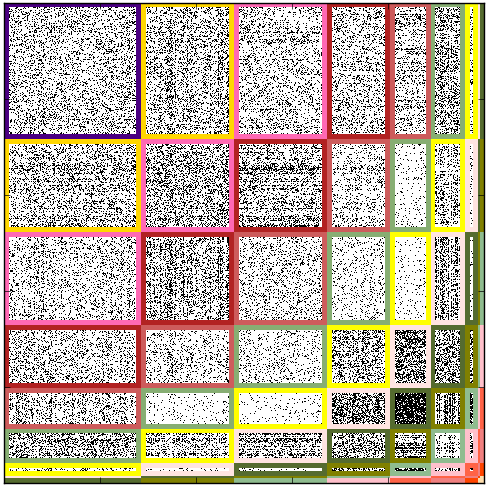
\includegraphics[width=2.94cm, height=3cm]{img/M_g_peaks/figure_6}
	\endminipage
		\minipage{0.17\textwidth}
	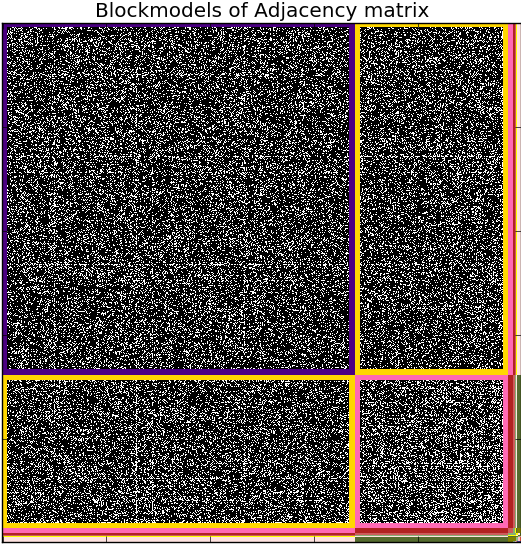
\includegraphics[width=2.94cm, height=3cm]{img/M_g_power_law/figure_6}
	\endminipage
	\minipage{0.17\textwidth}
	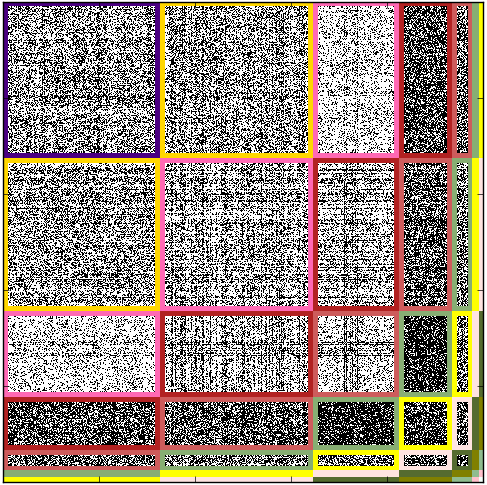
\includegraphics[width=2.94cm, height=3cm]{img/M_g_regular/figure_6}
	\endminipage
	%\vspace{-0.3cm}
    \vspace{0.3cm}
	\minipage{0.16\textwidth}
	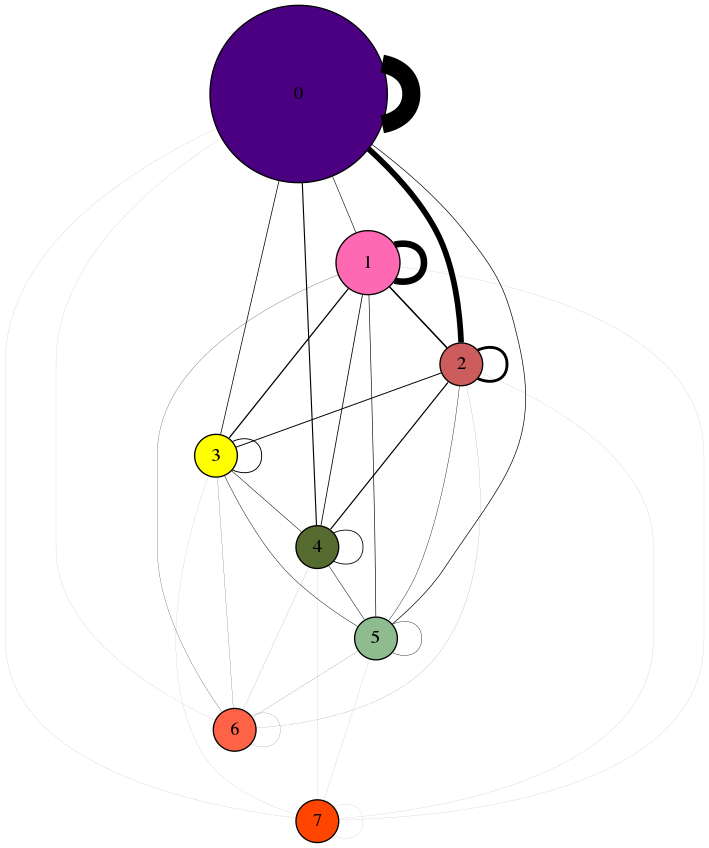
\includegraphics[width=3.5cm, height=4cm]{img/M_g_peaks/graph_dot}
	\endminipage
		\minipage{0.16\textwidth}
	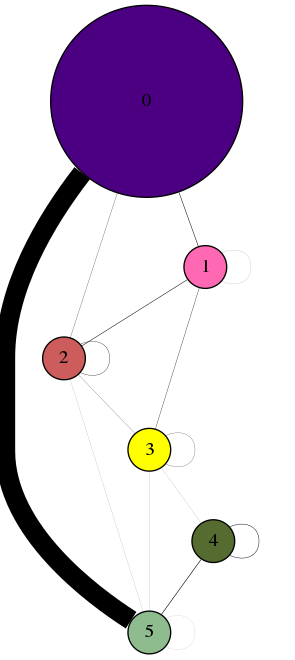
\includegraphics[width=3.5cm, height=4cm]{img/M_g_power_law/graph_dot} 
	\endminipage
	\minipage{0.16\textwidth}
	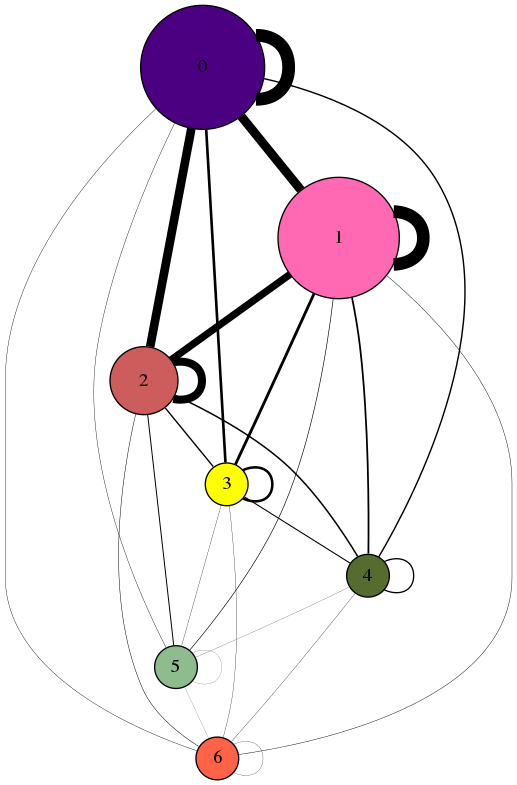
\includegraphics[width=3.5cm, height=4cm]{img/M_g_regular/graph_dot}
	\endminipage
	\caption{Tree examples of generated network in different setting of IMMSB. We reorder the adjacency matrix (white dot are links, block dot are non-link) in th upper figure, and plot their associated bock model structure in the lower part. The block structure is represented in the lower plots where we represent inter-block and intra-block connection by respectively edges ans self-loop.  }
	\label{fig:gen_blocks}
\end{figure}


 We now turn to the burstiness effect.
